% Options for packages loaded elsewhere
\PassOptionsToPackage{unicode}{hyperref}
\PassOptionsToPackage{hyphens}{url}
\PassOptionsToPackage{dvipsnames,svgnames,x11names}{xcolor}
%
\documentclass[
  letterpaper,
  DIV=11,
  numbers=noendperiod]{scrartcl}

\usepackage{amsmath,amssymb}
\usepackage{iftex}
\ifPDFTeX
  \usepackage[T1]{fontenc}
  \usepackage[utf8]{inputenc}
  \usepackage{textcomp} % provide euro and other symbols
\else % if luatex or xetex
  \usepackage{unicode-math}
  \defaultfontfeatures{Scale=MatchLowercase}
  \defaultfontfeatures[\rmfamily]{Ligatures=TeX,Scale=1}
\fi
\usepackage{lmodern}
\ifPDFTeX\else  
    % xetex/luatex font selection
  \setmainfont[]{Inter}
  \setsansfont[]{Inter}
\fi
% Use upquote if available, for straight quotes in verbatim environments
\IfFileExists{upquote.sty}{\usepackage{upquote}}{}
\IfFileExists{microtype.sty}{% use microtype if available
  \usepackage[]{microtype}
  \UseMicrotypeSet[protrusion]{basicmath} % disable protrusion for tt fonts
}{}
\makeatletter
\@ifundefined{KOMAClassName}{% if non-KOMA class
  \IfFileExists{parskip.sty}{%
    \usepackage{parskip}
  }{% else
    \setlength{\parindent}{0pt}
    \setlength{\parskip}{6pt plus 2pt minus 1pt}}
}{% if KOMA class
  \KOMAoptions{parskip=half}}
\makeatother
\usepackage{xcolor}
\setlength{\emergencystretch}{3em} % prevent overfull lines
\setcounter{secnumdepth}{5}
% Make \paragraph and \subparagraph free-standing
\ifx\paragraph\undefined\else
  \let\oldparagraph\paragraph
  \renewcommand{\paragraph}[1]{\oldparagraph{#1}\mbox{}}
\fi
\ifx\subparagraph\undefined\else
  \let\oldsubparagraph\subparagraph
  \renewcommand{\subparagraph}[1]{\oldsubparagraph{#1}\mbox{}}
\fi


\providecommand{\tightlist}{%
  \setlength{\itemsep}{0pt}\setlength{\parskip}{0pt}}\usepackage{longtable,booktabs,array}
\usepackage{calc} % for calculating minipage widths
% Correct order of tables after \paragraph or \subparagraph
\usepackage{etoolbox}
\makeatletter
\patchcmd\longtable{\par}{\if@noskipsec\mbox{}\fi\par}{}{}
\makeatother
% Allow footnotes in longtable head/foot
\IfFileExists{footnotehyper.sty}{\usepackage{footnotehyper}}{\usepackage{footnote}}
\makesavenoteenv{longtable}
\usepackage{graphicx}
\makeatletter
\def\maxwidth{\ifdim\Gin@nat@width>\linewidth\linewidth\else\Gin@nat@width\fi}
\def\maxheight{\ifdim\Gin@nat@height>\textheight\textheight\else\Gin@nat@height\fi}
\makeatother
% Scale images if necessary, so that they will not overflow the page
% margins by default, and it is still possible to overwrite the defaults
% using explicit options in \includegraphics[width, height, ...]{}
\setkeys{Gin}{width=\maxwidth,height=\maxheight,keepaspectratio}
% Set default figure placement to htbp
\makeatletter
\def\fps@figure{htbp}
\makeatother

\usepackage{amsmath, xparse}
\usepackage{fancyvrb, fvextra}
\usepackage{graphicx}
\usepackage{bm}
\usepackage{svg}
\usepackage{listings}
\usepackage{tikz}
\usepackage{multicol}
\usepackage{xifthen}
\DefineVerbatimEnvironment{Highlighting}{Verbatim}{breaklines,commandchars=\\\{\}}
\lstset{basicstyle=\ttfamily\footnotesize,breaklines=true}
\newcommand\encircle[1]{%
  \tikz[baseline=(X.base)]
    \node (X) [draw, shape=circle, inner sep=0] {\strut #1};}
\KOMAoption{captions}{tableheading}
\makeatletter
\makeatother
\makeatletter
\makeatother
\makeatletter
\@ifpackageloaded{caption}{}{\usepackage{caption}}
\AtBeginDocument{%
\ifdefined\contentsname
  \renewcommand*\contentsname{Table of contents}
\else
  \newcommand\contentsname{Table of contents}
\fi
\ifdefined\listfigurename
  \renewcommand*\listfigurename{List of Figures}
\else
  \newcommand\listfigurename{List of Figures}
\fi
\ifdefined\listtablename
  \renewcommand*\listtablename{List of Tables}
\else
  \newcommand\listtablename{List of Tables}
\fi
\ifdefined\figurename
  \renewcommand*\figurename{Figure}
\else
  \newcommand\figurename{Figure}
\fi
\ifdefined\tablename
  \renewcommand*\tablename{Table}
\else
  \newcommand\tablename{Table}
\fi
}
\@ifpackageloaded{float}{}{\usepackage{float}}
\floatstyle{ruled}
\@ifundefined{c@chapter}{\newfloat{codelisting}{h}{lop}}{\newfloat{codelisting}{h}{lop}[chapter]}
\floatname{codelisting}{Listing}
\newcommand*\listoflistings{\listof{codelisting}{List of Listings}}
\makeatother
\makeatletter
\@ifpackageloaded{caption}{}{\usepackage{caption}}
\@ifpackageloaded{subcaption}{}{\usepackage{subcaption}}
\makeatother
\makeatletter
\@ifpackageloaded{tcolorbox}{}{\usepackage[skins,breakable]{tcolorbox}}
\makeatother
\makeatletter
\@ifundefined{shadecolor}{\definecolor{shadecolor}{rgb}{.97, .97, .97}}
\makeatother
\makeatletter
\makeatother
\makeatletter
\makeatother
\ifLuaTeX
  \usepackage{selnolig}  % disable illegal ligatures
\fi
\IfFileExists{bookmark.sty}{\usepackage{bookmark}}{\usepackage{hyperref}}
\IfFileExists{xurl.sty}{\usepackage{xurl}}{} % add URL line breaks if available
\urlstyle{same} % disable monospaced font for URLs
\hypersetup{
  colorlinks=true,
  linkcolor={blue},
  filecolor={Maroon},
  citecolor={Blue},
  urlcolor={Blue},
  pdfcreator={LaTeX via pandoc}}

\author{}
\date{}

\begin{document}
\begin{titlepage}

    \newcommand{\HRule}{\rule{\linewidth}{0.5mm}}
    
    \center
    
    \vspace{10cm}

    \textsc{\LARGE Gwinnett School of Math, Science, and Technology }\\[0.3cm]
    
    \vspace{0.5cm}

    \HRule \\[0.4cm]
    { \huge \bfseries AP Physics: Mechanics/Electricity \& Magnetism Notes}\\[0.03cm]
    \HRule \\[1.5cm]
    
    \begin{minipage}{0.4\textwidth}
    \begin{flushleft} \Large
    Anish Goyal \\3rd/4th Period
    \end{flushleft}
    \end{minipage}
    ~
    \begin{minipage}{0.4\textwidth}
    \begin{flushright} \Large
    Jeffrey Burmester\\Educator
    \end{flushright}
    \end{minipage}\\[1cm]
    
    {\huge 2023-2024}\\[1cm]
    
    
\includegraphics{img/logo.png}\\
    \vfill
    \end{titlepage}
\newpage

\ifdefined\Shaded\renewenvironment{Shaded}{\begin{tcolorbox}[interior hidden, enhanced, borderline west={3pt}{0pt}{shadecolor}, frame hidden, breakable, sharp corners, boxrule=0pt]}{\end{tcolorbox}}\fi

\renewcommand*\contentsname{Table of Contents}
{
\hypersetup{linkcolor=}
\setcounter{tocdepth}{4}
\tableofcontents
}
\newpage{}

\hypertarget{kinematics}{%
\section{Kinematics}\label{kinematics}}

\hypertarget{variables}{%
\subsection{Variables}\label{variables}}

\hypertarget{position}{%
\subsubsection{\texorpdfstring{\textbf{Position}}{Position}}\label{position}}

\begin{itemize}
\tightlist
\item
  Typically given by the variable \(x\)
\end{itemize}

\hypertarget{time}{%
\subsubsection{\texorpdfstring{\textbf{Time}}{Time}}\label{time}}

\begin{itemize}
\tightlist
\item
  Typically given by the variables \(t\)
\end{itemize}

\hypertarget{displacement}{%
\subsubsection{\texorpdfstring{\textbf{Displacement}}{Displacement}}\label{displacement}}

\begin{itemize}
\tightlist
\item
  Defined as the change in position (\(X_f - X_i\))
\item
  Given by the variable \(\Delta x\)
\end{itemize}

\hypertarget{distance}{%
\subsubsection{\texorpdfstring{\textbf{Distance}}{Distance}}\label{distance}}

\begin{itemize}
\tightlist
\item
  You have to take the magnitude of vectors for every time you change
  position
\item
  \(S = |x_2 - x_1| + |x_1 - x_0| + ...\)
\end{itemize}

\hypertarget{average-velocity}{%
\subsubsection{\texorpdfstring{\textbf{Average
Velocity}}{Average Velocity}}\label{average-velocity}}

\begin{itemize}
\tightlist
\item
  Defined as the change in displacement over time
\item
  \(\frac{\Delta x}{\Delta t} = V_\text{avg} = \bar{V}\)
\end{itemize}

\hypertarget{velocity}{%
\subsubsection{\texorpdfstring{\textbf{Velocity}}{Velocity}}\label{velocity}}

\begin{itemize}
\tightlist
\item
  Defined as the change in displacement as time approaches 0
\item
  \(\lim_{\Delta t \to 0} \frac{\Delta x}{\Delta t} = \frac{dx}{dt} = V\)
\end{itemize}

\hypertarget{average-acceleration}{%
\subsubsection{\texorpdfstring{\textbf{Average
Acceleration}}{Average Acceleration}}\label{average-acceleration}}

\begin{itemize}
\tightlist
\item
  Defined as the change in velocity over time
\item
  \(\frac{\Delta V}{\Delta t} = A_\text{avg} = \bar{A}\)
\end{itemize}

\hypertarget{acceleration}{%
\subsubsection{\texorpdfstring{\textbf{Acceleration}}{Acceleration}}\label{acceleration}}

\begin{itemize}
\tightlist
\item
  Defined as the change in velocity as time approaches 0
\item
  \(a = \lim_{\Delta t \to 0} \frac{\Delta V}{\Delta t} = \frac{dV}{dt} = \frac{d^2x}{dt^2}\)
\end{itemize}

\hypertarget{speed}{%
\subsubsection{\texorpdfstring{\textbf{Speed}}{Speed}}\label{speed}}

\begin{itemize}
\tightlist
\item
  \(\text{Speed} = \frac{S}{t}\)
\item
  Alternatively, when referring to vectors:
  \(\text{Speed} = ||\vec{V}||\)
\end{itemize}

\hypertarget{velocity-and-position-definitions-0803-homework}{%
\subsection{Velocity and Position Definitions (08/03
Homework)}\label{velocity-and-position-definitions-0803-homework}}

\hypertarget{problem-1}{%
\subsubsection{Problem 1}\label{problem-1}}

The position versus time for a certain particle moving along the x axis
is shown in the figure below. Find the average velocity in the following
time intervals.

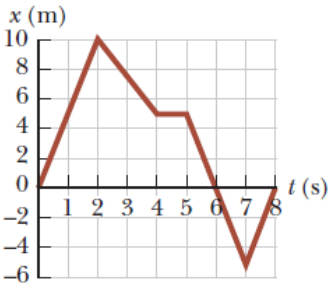
\includegraphics{img/Kinematics Velocity and Position HW/problem1.png}

\begin{enumerate}
\def\labelenumi{(\alph{enumi})}
\tightlist
\item
  0 to 2s
\end{enumerate}

\begin{itemize}
\tightlist
\item
  \(\frac{10-0}{2-0} = \frac{10}{2} = 5.000\) m/s
\end{itemize}

\begin{enumerate}
\def\labelenumi{(\alph{enumi})}
\setcounter{enumi}{1}
\tightlist
\item
  0 to 4s
\end{enumerate}

\begin{itemize}
\tightlist
\item
  \(\frac{5-0}{4-0}=\frac{5}{4}=1.250\) m/s
\end{itemize}

\begin{enumerate}
\def\labelenumi{(\alph{enumi})}
\setcounter{enumi}{2}
\tightlist
\item
  2 to 6s
\end{enumerate}

\begin{itemize}
\tightlist
\item
  \(\frac{0-10}{6-2}=\frac{-10}{4}=-2.500\) m/s
\end{itemize}

\begin{enumerate}
\def\labelenumi{(\alph{enumi})}
\setcounter{enumi}{3}
\tightlist
\item
  1 to 7s
\end{enumerate}

\begin{itemize}
\tightlist
\item
  \(\frac{-5-5}{7-1}=\frac{-10}{6}=-1.667\) m/s
\end{itemize}

\begin{enumerate}
\def\labelenumi{(\alph{enumi})}
\setcounter{enumi}{4}
\tightlist
\item
  0 to 7s
\end{enumerate}

\begin{itemize}
\tightlist
\item
  \(\frac{-5-0}{7-0}=\frac{-5}{7}=-0.714\) s
\end{itemize}

\hypertarget{problem-2}{%
\subsubsection{Problem 2}\label{problem-2}}

A person walks first at a constant speed of \(4.80\) m/s along a
straight line from point \encircle{$A$} to point \encircle{$B$} and then
back along the line from \encircle{$B$} to \encircle{$A$} at a constant
speed of \(2.90\) m/s.

\begin{enumerate}
\def\labelenumi{(\alph{enumi})}
\tightlist
\item
  What is her average speed over the entire trip?
\end{enumerate}

\begin{align*}
\text{Average speed} &= \frac{d_{AB}+d_{BA}}{t_{AB}+t_{BA}} \\
d &= d_{AB} = d_{BA} \\
t_{AB} &= \frac{d}{V_{AB}} \\
t{BA} &= \frac{d}{V_{BA}} \\
\therefore \text{ Average speed} &= \frac{d+d}{\frac{d}{V_{AB}}+\frac{d}{V_{BA}}} \\
&= \frac{2d(V_{AB})(V_{BA})}{2d} \\
&= \frac{2(V_{AB})(V_{BA})}{V_{AB}+V_{BA}} \\
&= 2\left[\frac{(4.80)(2.90)}{4.80+2.90}\right] \\
&= 3.615
\end{align*}

\begin{enumerate}
\def\labelenumi{(\alph{enumi})}
\setcounter{enumi}{1}
\tightlist
\item
  What is her average velocity over the entire trip?
\end{enumerate}

\begin{itemize}
\tightlist
\item
  Since her displacement is 0, her average velocity is also 0.
\end{itemize}

\newpage{}

\hypertarget{problem-3}{%
\subsubsection{Problem 3}\label{problem-3}}

A position-time graph for a particle moving along the x axis is shown in
the figure below.

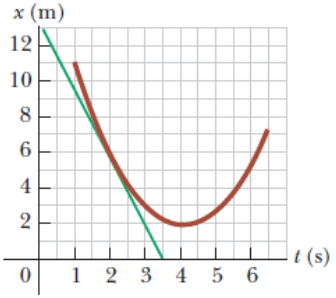
\includegraphics{img/Kinematics Velocity and Position HW/problem3.png}

\begin{enumerate}
\def\labelenumi{(\alph{enumi})}
\tightlist
\item
  Find the average velocity in the time interval \(t = 2.00\) s to
  \(t = 3.50\) s.
\end{enumerate}

\begin{itemize}
\tightlist
\item
  \(\frac{2-6}{3.5-2}=\frac{-4}{1.5}=-2.667\) m/s
\end{itemize}

\begin{enumerate}
\def\labelenumi{(\alph{enumi})}
\setcounter{enumi}{1}
\tightlist
\item
  Determine the instantaneous velocity at \(t = 2\) s (where the tangent
  line touches the curve) by measuring the slope of the tangent line
  shown in the graph.
\end{enumerate}

\begin{itemize}
\tightlist
\item
  \(\frac{2-12}{3.5-0} = \frac{-10}{3.5} = -3.714\) m/s
\end{itemize}

\begin{enumerate}
\def\labelenumi{(\alph{enumi})}
\setcounter{enumi}{2}
\tightlist
\item
  At what value of \(t\) is the velocity zero?
\end{enumerate}

\begin{itemize}
\tightlist
\item
  4.000 s
\end{itemize}

\newpage{}

\hypertarget{problem-4}{%
\subsubsection{Problem 4}\label{problem-4}}

A person takes a trip, driving with a constant speed of \(91.5\) km/h,
except for a \(24.0\)-min rest stop. The person's average speed is
\(71.6\) km/h.

\begin{enumerate}
\def\labelenumi{(\alph{enumi})}
\tightlist
\item
  How much time is spent on the trip? \begin{align*}
  \bar{V} &= \frac{(\text{Time driving})*V_\text{driving}}{\text{Total time}} \\
  71.6 &= \cfrac{(t-\frac{24}{60})\cdot 91.5}{t} \\
  71.6t &= (t-\frac{24}{60})\cdot 91.5 \\
  \frac{71.6}{91.5}t &= t-\frac{24}{60} \\
  \frac{71.6}{91.5}t - t &= -\frac{24}{60} \\
  \frac{71.6}{91.5}t - \frac{91.5}{91.5}t &= -\frac{24}{60} \\
  -\frac{19.9}{91.5}t &= -\frac{24}{60} \\
  t &= -\frac{24}{60}\cdot -\frac{91.5}{19.9} \\
  t &= 1.839 \text{ hours}
  \end{align*}
\item
  How far does the person travel?
\end{enumerate}

\begin{itemize}
\tightlist
\item
  \(d = \bar{V}\cdot t = (71.6)(1.839) = 131.6\) km
\end{itemize}

\newpage{}

\hypertarget{derivative-relationships}{%
\subsection{Derivative Relationships}\label{derivative-relationships}}

\hypertarget{acceleration-and-velocity}{%
\subsubsection{\texorpdfstring{\textbf{Acceleration and
Velocity}}{Acceleration and Velocity}}\label{acceleration-and-velocity}}

\begin{itemize}
\tightlist
\item
  \(a = \frac{dV}{dt}\)
\item
  \(V = \frac{dx}{dt}\)
\item
  \(\int_{V_0}^{V} dV = \int_{0}^{t} a \ dt\)
\item
  \(V\rvert_{V_0}^{V} = a\rvert_{0}^{t}\)
\item
  \(V - V_0 = at\)
\item
  \(V = at + V_0\)
\end{itemize}

\hypertarget{acceleration-and-position}{%
\subsubsection{\texorpdfstring{\textbf{Acceleration and
Position}}{Acceleration and Position}}\label{acceleration-and-position}}

\begin{itemize}
\tightlist
\item
  \(V = \frac{dx}{dt}\)
\item
  \(\int_{0}^{x} V dt = \int_{0}^{t} at + V_0 \ dt\)
\item
  \(x\rvert_{0}^{x} = \frac{1}{2}at^2 + V_0t\rvert_{0}^{t}\)
\item
  \(x = \frac{1}{2}at^2 + V_0t\)
\end{itemize}

\emph{If initial time or position is not zero:}

\begin{itemize}
\tightlist
\item
  \(x-x_0 = V_0(t-t_0) + \frac{1}{2}a(t-t_0)^2\)
\end{itemize}

\hypertarget{given-x4t4---6t-find-a-when-t2.}{%
\subsubsection{\texorpdfstring{Given \(x=4t^4 - 6t\), find \(a\) when
\(t=2\).}{Given x=4t\^{}4 - 6t, find a when t=2.}}\label{given-x4t4---6t-find-a-when-t2.}}

\begin{align*}
\frac{dx}{dt} &= 16t^3 - 6 \\
\frac{d^2x}{dt^2} &= 48t^2 \\
a &= 48(2)^2 \\
a &= 192
\end{align*}

\hypertarget{practice-with-1-d-kinematic-equations-moderate}{%
\subsection{Practice with 1-D Kinematic Equations
(moderate)}\label{practice-with-1-d-kinematic-equations-moderate}}

\hypertarget{problem-1-1}{%
\subsubsection{Problem 1}\label{problem-1-1}}

A world-class sprinter can burst out of the blocks to essentially top
speed (of about \(11.5\) m/s) in the first \(15.0\)m of the race. What
is the average acceleration of this sprinter and how long does it take
her to reach that speed (she accelerates uniformly)?

\hypertarget{problem-2-1}{%
\subsubsection{Problem 2}\label{problem-2-1}}

A car slows down from a speed of \(25.0\)m/s to rest in \(5.0\)s. How
far did it travel in that time?

\hypertarget{problem-3-1}{%
\subsubsection{Problem 3}\label{problem-3-1}}

In coming to a stop, a car leaves skid marks 80m long on the highway.
Assuming a deceleration of \(7.00 \text{m/s}^2\), estimate the speed of
the car just before braking.

\hypertarget{problem-4-1}{%
\subsubsection{Problem 4}\label{problem-4-1}}

A car traveling \(45\)km/h slows down at a constant
\(0.50 \text{m/s}^2\) just by ``letting up on the gas.'' Calculate:

\begin{enumerate}
\def\labelenumi{(\alph{enumi})}
\tightlist
\item
  the distance the car coasts before it stops
\item
  the time it takes to stop
\item
  the distance it travels during the first and fifth seconds
\end{enumerate}

\hypertarget{problem-5}{%
\subsubsection{Problem 5}\label{problem-5}}

A car traveling at \(90\)km/h strikes a tree. The front end of the car
compresses and the driver comes to rest after traveling \(0.80\)m. What
was the average acceleration of the driver during the collision? Express
the answer in terms of ``g's,'' where
\(1.00\text{g} = 9.80 \text{m/s}^2\)

\hypertarget{problem-6}{%
\subsubsection{Problem 6}\label{problem-6}}

Determine the stopping distances for an automobile with ana initial
speed of 90km/h and human reaction time of 1.0s:

\begin{enumerate}
\def\labelenumi{(\alph{enumi})}
\tightlist
\item
  for \(a =-4.0 \text{m/s}^2\)
\item
  for \(a = -8.0 \text{m/s}^2\)
\end{enumerate}

\hypertarget{acceleration-definitions-0804-homework}{%
\subsection{Acceleration Definitions (08/04
Homework)}\label{acceleration-definitions-0804-homework}}

\hypertarget{problem-1-2}{%
\subsubsection{Problem 1}\label{problem-1-2}}

A \(48.0\) g Super Ball traveling at \(29.0\) m/s bounces off a brick
wall and rebounds at \(18.0\) m/s. A high-speed camera records this
event. If the ball is in contact with the wall for \(4.05\) ms, what is
the magnitude of the average acceleration of the ball during this time
interval?

\begin{itemize}
\tightlist
\item
  \(a = \left|\frac{-18-29}{0.00405} = 11604.938\right|\) m/s\(^2\)
\end{itemize}

\newpage{}

\hypertarget{problem-2-2}{%
\subsubsection{Problem 2}\label{problem-2-2}}

A child rolls a marble on a bent track that is 100 cm long as shown in
the figure below. We use \(x\) to represent the position of the marble
along the track. On the horizontal sections from \(x=0\) to \(x=20\) cm
and from \(x=40\) to \(x=60\) cm, the marble rolls with constant speed.
On the sloping sections, the marble's speed changes steadily. At the
places where the slope changes, the marble stays on the track and does
not undergo any sudden changes in speed. The child gives the marble some
initial speed at \(x=0\) and \(t=0\) and then watches it roll to
\(x=90\) cm, where it turns around, eventually returning to \(x=0\) with
the same speed with which the child released it. Prepare graphs of \(x\)
versus \(t, v_x\) versus \(t\), and \(a_x\) versus \(t\), with their
time axes identical, to show the motion of the marble. You will not be
able to place any numbers other than zero on the horizontal axis or on
the velocity and acceleration axes, but show the correct graph shapes.

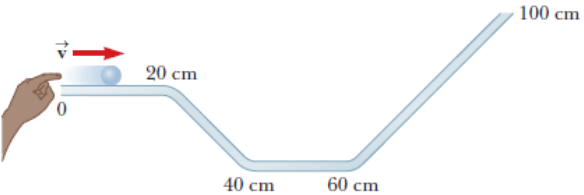
\includegraphics{img/Acceleration Definitions HW/problem1.png}

\newpage{}

\begin{figure}[!htb]
   \begin{minipage}{0.48\textwidth}
     \centering
     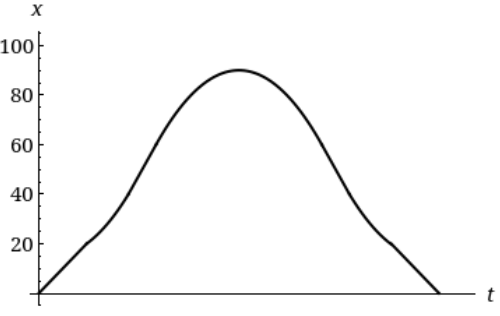
\includegraphics[width=\linewidth]{img/Acceleration Definitions HW/xversust.png}
     \caption*{$x$ versus $t$}
   \end{minipage}\hfill
   \begin{minipage}{0.48\textwidth}
     \centering
     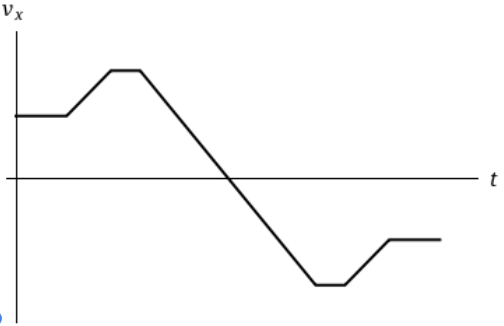
\includegraphics[width=\linewidth]{img/Acceleration Definitions HW/vxversust.png}
     \caption*{$V_x$ versus $t$}
   \end{minipage}
\end{figure}

\begin{figure}[!htb]
\begin{center}
   \begin{minipage}{0.48\textwidth}
     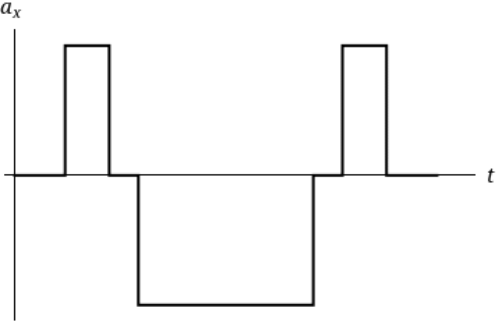
\includegraphics[width=\linewidth]{img/Acceleration Definitions HW/axversust.png}
     \caption*{$a_x$ versus $t$}
  \end{minipage}\hfill
\end{center}
\end{figure}

\newpage{}

\hypertarget{problem-3-2}{%
\subsubsection{Problem 3}\label{problem-3-2}}

A particle starts from rest and accelerates as shown in the figure
below.

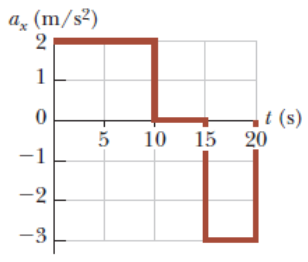
\includegraphics{img/Acceleration Definitions HW/problem3.png}

\begin{enumerate}
\def\labelenumi{(\alph{enumi})}
\tightlist
\item
  Determine the particle's speed at \(t = 10.0\) s.
\end{enumerate}

\begin{itemize}
\tightlist
\item
  \(\int_0^{10} a \ dt = 10 \cdot 2 = 20\) m/s
\end{itemize}

\begin{enumerate}
\def\labelenumi{(\alph{enumi})}
\setcounter{enumi}{1}
\tightlist
\item
  Determine the particle's speed at \(t = 20.0\) s?
\end{enumerate}

\begin{itemize}
\tightlist
\item
  \(\int_0^{20} a \ dt = 10 \cdot 2 + 5 \cdot (-3) = 20 - 15 = 5\) m/s
\end{itemize}

\begin{enumerate}
\def\labelenumi{(\alph{enumi})}
\setcounter{enumi}{2}
\tightlist
\item
  Determine the distance traveled in the first \(20.0\) s. (Enter your
  answer to one decimal places.)
\end{enumerate}

\begin{align*}
\Delta x \text{ from 0-10 seconds: }\frac{1}{2} \cdot 2 \cdot 10^2 &= 100 \\
\Delta x \text{ from 10-15 seconds: }20 \cdot 5 &= 100 \\
\Delta x \text{ from 15-20 seconds: } \frac{1}{2} \cdot -3 \cdot 5^2 + 20 \cdot 5 &= 62.5 \\
\therefore \Delta x &= 262.5 \text{ m}
\end{align*}

\hypertarget{problem-4-2}{%
\subsubsection{Problem 4}\label{problem-4-2}}

An object moves along the x axis according to the equation
\(x = 3.25t^2 − 2.00t + 3.00\), where \(x\) is in meters and \(t\) is in
seconds.

\begin{enumerate}
\def\labelenumi{(\alph{enumi})}
\tightlist
\item
  Determine the average speed between \(t = 1.70\) s and \(t = 3.30\) s.
\end{enumerate}

\begin{itemize}
\tightlist
\item
  \(\bar{V} = \frac{x(3.30)-x(1.70)}{t_1-t_0} = \frac{(3.25(3.30)^2-2(3.30)+3) - (3.25(1.70)^2-2(1.70)+3)}{3.30-1.70} = 14.25\)
  m/s
\end{itemize}

\begin{enumerate}
\def\labelenumi{(\alph{enumi})}
\setcounter{enumi}{1}
\tightlist
\item
  Determine the instantaneous speed at \(t = 1.70\) s.
\end{enumerate}

\begin{itemize}
\tightlist
\item
  \(V = \frac{dx}{dt} = 6.5(1.7)-2 = 9.05\) m/s
\end{itemize}

\begin{enumerate}
\def\labelenumi{(\alph{enumi})}
\setcounter{enumi}{2}
\tightlist
\item
  Determine the instantaneous speed at \(t = 3.30\) s.
\end{enumerate}

\begin{itemize}
\tightlist
\item
  \(V = \frac{dx}{dt} = 2(3.25)(3.3)-2 = 19.45\) m/s
\end{itemize}

\begin{enumerate}
\def\labelenumi{(\alph{enumi})}
\setcounter{enumi}{3}
\tightlist
\item
  Determine the average acceleration between \(t = 1.70 s\) and
  \(t = 3.30\) s.
\end{enumerate}

\begin{itemize}
\tightlist
\item
  \(\bar{a} = \frac{V(3.30)-V(1.70)}{t_1-t_0} = \frac{(2(3.25)(3.30)-2)-(2(3.25)(1.70)-2)}{3.30-1.70} = 6.5\)
  m/s\(^2\)
\end{itemize}

\begin{enumerate}
\def\labelenumi{(\alph{enumi})}
\setcounter{enumi}{4}
\tightlist
\item
  Determine the instantaneous acceleration at \(t = 1.70\) s.
\end{enumerate}

\begin{itemize}
\tightlist
\item
  \(a = \frac{dV}{dt} = 2(3.25) = 6.5\) m/s\(^2\)
\end{itemize}

\begin{enumerate}
\def\labelenumi{(\alph{enumi})}
\setcounter{enumi}{5}
\tightlist
\item
  Determine the instantaneous acceleration at \(t = 3.30\) s.
\end{enumerate}

\begin{itemize}
\tightlist
\item
  \(a = \frac{dV}{dt} = 2(3.25) = 6.5\) m/s\(^2\)
\end{itemize}

\begin{enumerate}
\def\labelenumi{(\alph{enumi})}
\setcounter{enumi}{6}
\tightlist
\item
  At what time is the object at rest?
\end{enumerate}

\begin{itemize}
\tightlist
\item
  0 = \(6.5t-2 \implies 0.308\) s
\end{itemize}



\end{document}
